\documentclass[aspectratio=169, 11pt]{beamer}

% ===== PACKAGES =====
\usepackage[utf8]{inputenc}
\usepackage[T5]{fontenc}
\usepackage[vietnamese,english]{babel}
\usepackage{amsmath, amssymb}
\usepackage{booktabs}
\usepackage{graphicx}
\usepackage{xcolor}
\usepackage{listings}
\usepackage{tikz}
\usetikzlibrary{positioning, arrows.meta}

\graphicspath{{../../}{./}}

% ===== THEME =====
\usetheme{Madrid}
\usecolortheme{default}
\definecolor{primaryblue}{RGB}{0,84,166}
\definecolor{softgray}{RGB}{245,247,250}
\definecolor{accentgreen}{RGB}{22,130,90}
\definecolor{accentorange}{RGB}{224,126,35}

\setbeamercolor{structure}{fg=primaryblue}
\setbeamercolor{title}{fg=white,bg=primaryblue}
\setbeamercolor{frametitle}{fg=white,bg=primaryblue}
\setbeamercolor{block title}{fg=white,bg=primaryblue}
\setbeamercolor{block body}{bg=softgray}
\setbeamertemplate{navigation symbols}{}
\setbeamertemplate{footline}[frame number]

% ===== LISTINGS =====
\lstdefinestyle{codestyle}{
  basicstyle=\ttfamily\scriptsize,
  breaklines=true,
  frame=single,
  rulecolor=\color{gray!40},
  backgroundcolor=\color{softgray},
  keywordstyle=\color{primaryblue}\bfseries,
  commentstyle=\color{accentgreen},
  stringstyle=\color{accentorange}
}
\lstset{style=codestyle}

% ===== META =====
\title[Tập thống trị tối thiểu]{Bài toán Tập Thống Trị Tối Thiểu}
\subtitle{Thiết kế, cài đặt và đánh giá thuật toán}
\author[Nhóm 5]{
  Hoàng Minh Quang -- 23001917\\
  Nguyễn Đức Quang -- 23001918\\
  Nguyễn Thành Tâm -- 23001929\\
  Nguyễn Thế Tài -- 23001926
}
\institute{Môn học: Thiết kế và Đánh giá thuật toán}
\date{Hà Nội, tháng 5 năm 2026}

\begin{document}
\selectlanguage{vietnamese}

% 1
\begin{frame}
  \titlepage
\end{frame}

% 2
\begin{frame}{Nội dung trình bày}
  \tableofcontents
\end{frame}

\section{Bài toán}

% 3
\begin{frame}{Đặt vấn đề}
  \begin{block}{Câu hỏi chính}
    Làm thế nào chọn ít điểm nhất trong một mạng lưới sao cho mọi điểm đều được phục vụ?
  \end{block}

  \begin{itemize}
    \item Đặt trạm phát sóng để phủ khu vực dân cư.
    \item Đặt đồn cảnh sát tại một số nút giao thông.
    \item Chọn máy chủ giám sát trong mạng máy tính.
    \item Chọn người đại diện trong mạng xã hội.
  \end{itemize}

  \vspace{0.2cm}
  Bài toán này được mô hình hóa bằng \textbf{Minimum Dominating Set}.
\end{frame}

% 4
\begin{frame}{Mô hình đồ thị}
  Cho đồ thị vô hướng, không trọng số:
  \[
    G=(V,E)
  \]

  \begin{itemize}
    \item $V$: tập đỉnh, biểu diễn các vị trí hoặc đối tượng.
    \item $E$: tập cạnh, biểu diễn quan hệ kề nhau hoặc có thể phục vụ trực tiếp.
    \item $N(v)$: tập láng giềng của đỉnh $v$.
    \item $N[v]=N(v)\cup\{v\}$: láng giềng đóng của $v$.
  \end{itemize}

  \begin{block}{Ý nghĩa}
    Nếu chọn đỉnh $v$, ta phủ được toàn bộ các đỉnh trong $N[v]$.
  \end{block}
\end{frame}

% 5
\begin{frame}{Định nghĩa tập thống trị}
  Một tập $D \subseteq V$ là \textbf{tập thống trị} nếu:
  \[
    \forall u \in V,\quad u\in D \ \text{hoặc}\ \exists v\in D: (u,v)\in E.
  \]

  Tương đương:
  \[
    \mathrm{cover}(D)=\bigcup_{v\in D}N[v]=V.
  \]

  \begin{block}{Bài toán tối ưu}
    Tìm tập thống trị $D^*$ có kích thước nhỏ nhất:
    \[
      |D^*|=\min\{|D|:\ D\subseteq V,\ \mathrm{cover}(D)=V\}.
    \]
  \end{block}
\end{frame}

% 6
\begin{frame}{Ví dụ minh họa}
  \centering
  \begin{tikzpicture}[
    node/.style={circle, draw=primaryblue, fill=white, thick, minimum size=8mm},
    chosen/.style={circle, draw=accentgreen, fill=accentgreen!18, thick, minimum size=8mm}
  ]
    \node[node] (0) at (0,0) {0};
    \node[chosen] (1) at (1.4,0) {1};
    \node[node] (2) at (2.8,0) {2};
    \node[chosen] (3) at (4.2,0) {3};
    \node[node] (4) at (5.6,0) {4};
    \draw[thick] (0)--(1)--(2)--(3)--(4);
  \end{tikzpicture}

  \vspace{0.5cm}
  Với đường đi $P_5$, chọn $D=\{1,3\}$:
  \[
    N[1]\cup N[3]=\{0,1,2\}\cup\{2,3,4\}=V.
  \]

  \begin{block}{Kết luận}
    $D=\{1,3\}$ là tập thống trị tối thiểu, vì một đỉnh không thể phủ cả 5 đỉnh.
  \end{block}
\end{frame}

% 7
\begin{frame}{Độ khó bài toán}
  \begin{itemize}
    \item Phiên bản quyết định: có tồn tại tập thống trị $D$ sao cho $|D|\leq k$ không?
    \item Bài toán thuộc NP vì có thể kiểm tra nghiệm trong thời gian đa thức.
    \item Bài toán là NP-complete ở dạng quyết định.
    \item Phiên bản tối ưu là NP-hard.
  \end{itemize}

  \begin{block}{Hệ quả}
    Khó có thuật toán đa thức luôn tìm nghiệm tối ưu cho mọi đồ thị tổng quát.
  \end{block}

  Vì vậy cần kết hợp:
  \begin{itemize}
    \item thuật toán chính xác cho đồ thị nhỏ;
    \item thuật toán xấp xỉ/heuristic cho đồ thị lớn.
  \end{itemize}
\end{frame}

\section{Thuật toán}

% 8
\begin{frame}{Các thuật toán trong project}
  \begin{table}
    \centering
    \begin{tabular}{p{3.1cm} p{3.2cm} p{2.6cm} p{2.4cm}}
      \toprule
      \textbf{Thuật toán} & \textbf{File} & \textbf{Loại} & \textbf{Tối ưu?} \\
      \midrule
      Vét cạn & \texttt{brute\_force.py} & Chính xác & Có \\
      Nhánh cận & \texttt{branch\_bound.py} & Chính xác & Có \\
      Tham lam & \texttt{greedy.py} & Xấp xỉ & Không \\
      ACO & \texttt{aco.py} & Metaheuristic & Không \\
      \bottomrule
    \end{tabular}
  \end{table}

  \begin{block}{Mục tiêu so sánh}
    Đánh giá sự đánh đổi giữa \textbf{độ chính xác}, \textbf{thời gian chạy} và \textbf{khả năng mở rộng}.
  \end{block}
\end{frame}

% 9
\begin{frame}[fragile]{Biểu diễn đồ thị trong chương trình}
  \begin{lstlisting}[language=Python]
adj = [
    {1, 2},     # neighbors of vertex 0
    {0, 3},     # neighbors of vertex 1
    {0, 4},     # neighbors of vertex 2
    {1, 5},     # neighbors of vertex 3
    {2, 6},     # neighbors of vertex 4
    {3, 6},     # neighbors of vertex 5
    {4, 5},     # neighbors of vertex 6
]
  \end{lstlisting}

  \begin{itemize}
    \item \texttt{adj[v]} là tập các đỉnh kề với $v$.
    \item Dùng \texttt{set} giúp hợp tập và hiệu tập dễ cài đặt.
    \item Kiểm tra nghiệm bằng cách tính tập đỉnh đã được phủ.
  \end{itemize}
\end{frame}
\begin{frame}{Thuật toán tham lam}
  \begin{block}{Ý tưởng}
    Mỗi bước chọn đỉnh phủ được nhiều đỉnh chưa phủ nhất.
  \end{block}

  Với mỗi đỉnh $v$, định nghĩa:
  \[
    gain(v)=|N[v]\setminus dominated|.
  \]

  Lặp đến khi phủ hết đồ thị:
  \begin{enumerate}
    \item Chọn $v$ có $gain(v)$ lớn nhất.
    \item Thêm $v$ vào $D$.
    \item Cập nhật $dominated \gets dominated \cup N[v]$.
  \end{enumerate}
\end{frame}

% 16
\begin{frame}{Đánh giá tham lam}
  \begin{columns}
    \begin{column}{0.48\textwidth}
      \begin{block}{Ưu điểm}
        \begin{itemize}
          \item Rất nhanh.
          \item Cài đặt đơn giản.
          \item Chạy được với đồ thị lớn.
          \item Có liên hệ với Set Cover.
        \end{itemize}
      \end{block}
    \end{column}
    \begin{column}{0.48\textwidth}
      \begin{block}{Nhược điểm}
        \begin{itemize}
          \item Không đảm bảo tối ưu.
          \item Có thể bị ảnh hưởng bởi lựa chọn cục bộ.
          \item Kết quả phụ thuộc cấu trúc đồ thị.
        \end{itemize}
      \end{block}
    \end{column}
  \end{columns}

  \vspace{0.4cm}
  \[
    T(n)= O(n(n+m)).
  \]
\end{frame}

% 10
\begin{frame}{Thuật toán vét cạn}
  \begin{block}{Ý tưởng}
    Thử tất cả tập con của $V$ theo thứ tự kích thước tăng dần.
  \end{block}

  \begin{enumerate}
    \item Với $k=1,2,\ldots,n$.
    \item Sinh mọi tập con $D$ có $|D|=k$.
    \item Nếu $\mathrm{cover}(D)=V$, trả về $D$.
  \end{enumerate}

  \begin{block}{Vì sao tối ưu?}
    Tập hợp lệ đầu tiên được tìm thấy có kích thước nhỏ nhất vì thuật toán đã thử hết mọi kích thước nhỏ hơn.
  \end{block}
\end{frame}
\begin{frame}{Chứng minh đúng đắn: vét cạn}
  \begin{block}{Tính hợp lệ}
    Thuật toán chỉ trả về $D$ sau khi kiểm tra $\mathrm{cover}(D)=V$.
  \end{block}

  \begin{block}{Tính tối ưu}
    Thuật toán xét các tập con theo kích thước tăng dần.
    Nếu trả về tập kích thước $k$, mọi tập kích thước nhỏ hơn $k$ đã được xét và đều không hợp lệ.
  \end{block}

  \begin{alertblock}{Kết luận}
    Vét cạn luôn trả về tập thống trị tối thiểu.
  \end{alertblock}
\end{frame}
% 11
\begin{frame}{Đánh giá vét cạn}
  \begin{columns}
    \begin{column}{0.48\textwidth}
      \begin{block}{Ưu điểm}
        \begin{itemize}
          \item Dễ hiểu, dễ cài đặt.
          \item Luôn tìm nghiệm tối ưu.
          \item Phù hợp làm chuẩn kiểm tra.
        \end{itemize}
      \end{block}
    \end{column}
    \begin{column}{0.48\textwidth}
      \begin{block}{Nhược điểm}
        \begin{itemize}
          \item Số tập con là $2^n$.
          \item Không dùng được cho đồ thị lớn.
          \item Trong project chỉ chạy với $n\leq16$.
        \end{itemize}
      \end{block}
    \end{column}
  \end{columns}

  \vspace{0.4cm}
  \[
    T(n)=O(2^n\cdot n)
  \]
\end{frame}

% 12
\begin{frame}{Thuật toán nhánh cận}
  \begin{block}{Ý tưởng}
    Vẫn tìm nghiệm tối ưu, nhưng cắt bỏ những nhánh chắc chắn không thể tốt hơn nghiệm hiện tại.
  \end{block}

  Tại một trạng thái:
  \begin{itemize}
    \item $D$: tập đỉnh đã chọn.
    \item $dominated$: tập đỉnh đã được phủ.
    \item Chọn một đỉnh chưa phủ $u$.
    \item Muốn phủ $u$, bắt buộc phải chọn một đỉnh trong $N[u]$.
  \end{itemize}

  Do đó ta chỉ phân nhánh theo các ứng viên trong $N[u]$.
\end{frame}

% 13
\begin{frame}{Cận dưới trong nhánh cận}
  Gọi $\Delta$ là bậc lớn nhất của đồ thị. Một đỉnh phủ tối đa $\Delta+1$ đỉnh.

  Nếu còn $r$ đỉnh chưa được phủ, số đỉnh cần chọn thêm ít nhất là:
  \[
    LB=\left\lceil \frac{r}{\Delta+1}\right\rceil.
  \]

  Cắt nhánh khi:
  \[
    |D| + LB \geq |D_{\mathrm{best}}|.
  \]

  \begin{block}{Cận trên ban đầu}
    Project dùng nghiệm tham lam làm $D_{\mathrm{best}}$ ban đầu để cắt nhánh sớm hơn.
  \end{block}
\end{frame}
\begin{frame}{Chứng minh đúng đắn: nhánh cận}
  \begin{block}{Lập luận phân nhánh}
    Nếu $u$ chưa được phủ, nghiệm cuối cùng bắt buộc phải chọn $u$ hoặc một láng giềng của $u$.
    Do đó chỉ cần phân nhánh trên $N[u]$.
  \end{block}

  \begin{block}{Lập luận cắt nhánh}
    Nếu $|D|+LB \geq |D_{\mathrm{best}}|$, mọi nghiệm trong nhánh này không thể tốt hơn nghiệm tốt nhất hiện có.
  \end{block}

  \begin{alertblock}{Kết luận}
    Nhánh cận không bỏ sót nghiệm tối ưu và luôn trả về nghiệm tối ưu.
  \end{alertblock}
\end{frame}
% 14
\begin{frame}{Đánh giá nhánh cận}
  \begin{columns}
    \begin{column}{0.48\textwidth}
      \begin{block}{Ưu điểm}
        \begin{itemize}
          \item Luôn tìm nghiệm tối ưu.
          \item Nhanh hơn vét cạn trong thực tế.
          \item Tận dụng được cận trên tham lam.
        \end{itemize}
      \end{block}
    \end{column}
    \begin{column}{0.48\textwidth}
      \begin{block}{Nhược điểm}
        \begin{itemize}
          \item Worst-case vẫn hàm mũ.
          \item Phụ thuộc cấu trúc đồ thị.
          \item Trong project chỉ chạy với $n\leq30$.
        \end{itemize}
      \end{block}
    \end{column}
  \end{columns}

  \vspace{0.4cm}
  \[
    T(n)=O(2^n)\ \text{trong trường hợp xấu}
  \]
\end{frame}

% 15


% 17
\begin{frame}{Thuật toán ACO}
  \begin{block}{Ý tưởng}
    Mỗi kiến xây dựng một nghiệm bằng cách chọn đỉnh theo xác suất dựa trên kinh nghiệm và lợi ích hiện tại.
  \end{block}

  Hai thành phần chính:
  \begin{itemize}
    \item Pheromone $\tau(v)$: đỉnh $v$ thường xuất hiện trong nghiệm tốt.
    \item Heuristic $\eta(v)$: số đỉnh mới được phủ nếu chọn $v$.
  \end{itemize}

  Xác suất chọn:
  \[
    P(v)=\frac{\tau(v)^\alpha \eta(v)^\beta}
    {\sum_{u}\tau(u)^\alpha \eta(u)^\beta}.
  \]
\end{frame}

% 18
\begin{frame}{ACO trong project}
  Quy trình chính:
  \begin{enumerate}
    \item Khởi tạo pheromone đều nhau.
    \item Mỗi kiến xây dựng một tập thống trị.
    \item Áp dụng local search để xóa đỉnh dư thừa.
    \item Pheromone bốc hơi với hệ số $\rho$.
    \item Bồi đắp pheromone theo các nghiệm tốt.
    \item Lặp nhiều vòng và lưu nghiệm tốt nhất.
  \end{enumerate}

  \begin{block}{Độ phức tạp}
    \[
      O(iterations \cdot ants \cdot n^2)
    \]
  \end{block}
\end{frame}

\section{Chứng minh và phân tích}

% 19


% 20


% 21
\begin{frame}{Bảng so sánh lý thuyết}
  \begin{table}
    \centering
    \small
    \begin{tabular}{p{2.7cm} p{3.2cm} p{2.2cm} p{4.0cm}}
      \toprule
      \textbf{Thuật toán} & \textbf{Độ phức tạp} & \textbf{Tối ưu?} & \textbf{Phù hợp} \\
      \midrule
      Vét cạn & $O(2^n n)$ & Có & Đồ thị rất nhỏ, kiểm chứng nghiệm \\
      Nhánh cận & $O(2^n)$ worst-case & Có & Đồ thị nhỏ/trung bình \\
      Tham lam & $O(n(n+m))$ & Không & Đồ thị lớn, cần tốc độ \\
      ACO & $O(TAn^2)$ & Không & Đồ thị lớn, muốn nghiệm tốt hơn tham lam \\
      \bottomrule
    \end{tabular}
  \end{table}
\end{frame}

\section{Thực nghiệm}

% 22
\begin{frame}{Thiết kế thực nghiệm}
  Benchmark dùng đồ thị ngẫu nhiên $G(n,p)$.

  \begin{itemize}
    \item $n \in \{8,12,16,20,30,50,100\}$.
    \item $p \in \{0.05,0.10,0.30,0.50\}$.
    \item Seed: $0,1,2$.
    \item Vét cạn chạy với $n\leq16$.
    \item Nhánh cận chạy với $n\leq30$.
    \item Tham lam và ACO chạy với mọi $n$.
  \end{itemize}

  \begin{block}{Chỉ số đánh giá}
    Thời gian chạy, kích thước nghiệm $|D|$, tính hợp lệ và gap so với tối ưu.
  \end{block}
\end{frame}

% 23
\begin{frame}{Kết quả: thời gian thực thi}
  \centering
  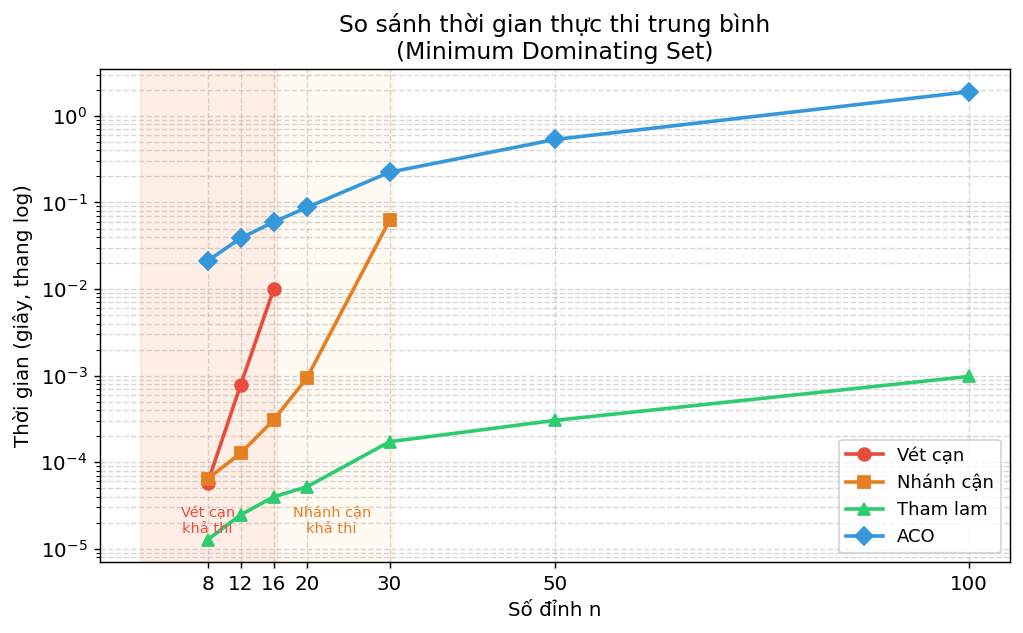
\includegraphics[width=0.86\textwidth]{results/plots/time_comparison.png}

  \vspace{0.2cm}
  \small
  Tham lam nhanh nhất; vét cạn tăng rất nhanh; nhánh cận cải thiện đáng kể so với vét cạn; ACO chậm hơn tham lam do nhiều kiến và nhiều vòng lặp.
\end{frame}

% 24
\begin{frame}{Kết quả: chất lượng nghiệm}
  \centering
  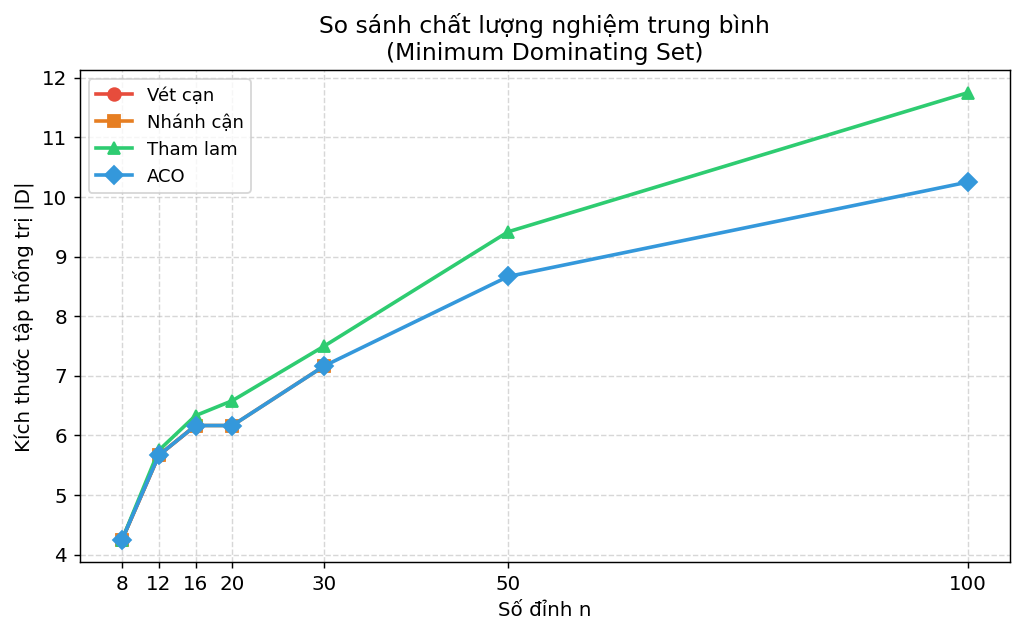
\includegraphics[width=0.86\textwidth]{results/plots/size_comparison.png}

  \vspace{0.2cm}
  \small
  Đồ thị càng dày thì tập thống trị càng nhỏ. ACO có thể cho nghiệm nhỏ hơn tham lam ở một số đồ thị lớn.
\end{frame}

% 25
\begin{frame}{Nhận xét thực nghiệm}
  \begin{itemize}
    \item Trên các đồ thị nhỏ, vét cạn và nhánh cận đều cho gap bằng 0.
    \item Nhánh cận thường nhanh hơn vét cạn nhờ cắt nhánh.
    \item Tham lam có tốc độ rất tốt, phù hợp khi cần kết quả nhanh.
    \item ACO tốn thời gian hơn nhưng thường cải thiện nghiệm ở đồ thị lớn/thưa.
    \item Khi mật độ cạnh tăng, số đỉnh cần chọn giảm rõ rệt.
  \end{itemize}

  \begin{block}{Đánh đổi chính}
    Chính xác tuyệt đối thường đi kèm chi phí lớn; heuristic nhanh hơn nhưng chấp nhận sai lệch.
  \end{block}
\end{frame}

\section{Kết luận}

% 26
\begin{frame}{Kết luận}
  \begin{table}
    \centering
    \small
    \begin{tabular}{p{3cm} p{8cm}}
      \toprule
      \textbf{Trường hợp} & \textbf{Nên dùng} \\
      \midrule
      $n \leq 16$ & Vét cạn: đơn giản, chắc chắn tối ưu. \\
      $16 < n \leq 30$ & Nhánh cận: vẫn tối ưu, nhanh hơn vét cạn. \\
      $n > 30$, ưu tiên tốc độ & Tham lam. \\
      $n > 30$, ưu tiên nghiệm tốt hơn & ACO hoặc ACO kết hợp tham lam/local search. \\
      \bottomrule
    \end{tabular}
  \end{table}

  \begin{block}{Kết quả đạt được}
    Project đã cài đặt, kiểm chứng và so sánh 4 hướng giải cho bài toán Minimum Dominating Set.
  \end{block}
\end{frame}

% 27
\begin{frame}{Hướng phát triển}
  \begin{itemize}
    \item Cải thiện cận dưới trong nhánh cận để cắt nhánh mạnh hơn.
    \item Tối ưu tham lam bằng hàng đợi ưu tiên.
    \item Thử thêm thuật toán genetic algorithm, simulated annealing hoặc local search nâng cao.
    \item Thực nghiệm trên dữ liệu thực tế: mạng giao thông, mạng xã hội, mạng máy tính.
    \item Mở rộng sang weighted dominating set và connected dominating set.
  \end{itemize}
\end{frame}

% 28
\begin{frame}
  \centering
  \Huge\textbf{Cảm ơn thầy/cô và các bạn đã lắng nghe!}

  \vspace{0.8cm}
  \Large Q \& A
\end{frame}

\end{document}
